% Skype network topology
% Author Fiandrino Claudio 2011
% http://claudiofiandrino.altervista.org/
\documentclass{article}
\usepackage{tikz}
\definecolor{violet}{cmyk}{0.79,0.88,0,0}

\tikzstyle{vertex}=[draw,circle,text=violet,minimum width=20pt]
\begin{document}
\begin{figure}[H]
  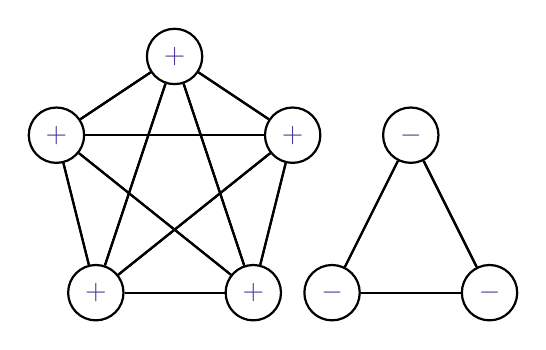
\begin{tikzpicture}[auto, thick]
\tikzstyle{vertex}=[draw,circle,text=violet,minimum width=20pt]
  \foreach \place/\name in {{(0,0)/a},
                            {(-0.5,2)/b},
                            {(2,0)/c},
                            {(2.5,2)/d},
                            {(1,3)/e}}
    \node[vertex] (\name) at \place {$+$};
  \foreach \place/\name in {{(3,0)/f},
                            {(5,0)/g},
                            {(4,2)/h}}
    \node[vertex] (\name) at \place {$-$};
  \foreach \source in {a,b,c,d,e}
    \foreach \dest in {a,b,c,d,e}
      \path (\source) edge (\dest);
  \foreach \source in {f,g,h}
    \foreach \dest in {f,g,h}
      \path (\source) edge (\dest);
\end{tikzpicture}
  \caption{${\cal G}(3,5)$}
\end{figure}

\begin{figure}[H]
  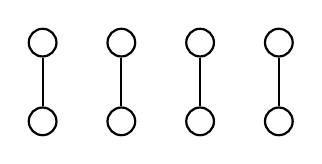
\begin{tikzpicture}[auto, thick]
\tikzstyle{vertex}=[draw,circle,text=violet,minimum width=10pt]
  \foreach \place/\name in {{(0,0)/a},
                            {(0,1)/b},
                            {(1,0)/c},
                            {(1,1)/d},
                            {(2,0)/e},
                            {(2,1)/f},
                            {(3,0)/g},
                            {(3,1)/h}}
    \node[vertex] (\name) at \place {};
  \foreach \source/\dest in {a/b,c/d,e/f,g/h}
      \path (\source) edge (\dest);
\end{tikzpicture}
  \caption{OTS(3,5)}
\end{figure}


\begin{figure}[H]
  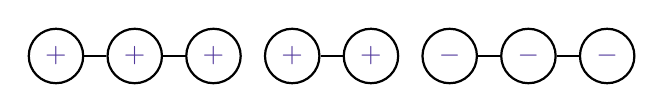
\begin{tikzpicture}[auto, thick]
\tikzstyle{vertex}=[draw,circle,text=violet,minimum width=15pt]
  \foreach \place/\name in {{(0,0)/a},
                            {(1,0)/b},
                            {(2,0)/c},
                            {(3,0)/g},
                            {(4,0)/h}}
    \node[vertex] (\name) at \place {$+$};
  \foreach \place/\name in {{(5,0)/d},
                            {(6,0)/e},
                            {(7,0)/f}}
    \node[vertex] (\name) at \place {$-$};
  \foreach \source/\dest in {a/b,b/c,d/e,e/f,g/h}
      \path (\source) edge (\dest);
\end{tikzpicture}
  \caption{notTS(3,5)}
\end{figure}

\begin{figure}[H]
  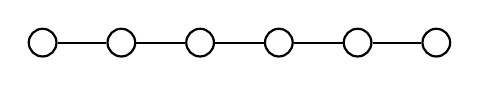
\begin{tikzpicture}[auto, thick]
\tikzstyle{vertex}=[draw,circle,text=violet,minimum width=10pt]
  \foreach \place/\name in {{(0,0)/a},
                            {(1,0)/b},
                            {(2,0)/c},
                            {(3,0)/d},
                            {(4,0)/e},
                            {(5,0)/f}}
    \node[vertex] (\name) at \place {};
  \foreach \source/\dest in {a/b,b/c,c/d,d/e,e/f}
      \path (\source) edge (\dest);
\end{tikzpicture}
  \caption{notTS(3,5)}
\end{figure}

\end{document}
